\documentclass[11pt,a4paper]{article}

% --- Packages ---
\usepackage[utf8]{inputenc}
\usepackage[T1]{fontenc}
\usepackage{lmodern}
\usepackage[margin=2.5cm]{geometry}
\usepackage{amsmath,amssymb}
\usepackage{booktabs}
\usepackage{array}
\usepackage{tabularx}
\usepackage{enumitem}
\usepackage{xcolor}
\usepackage{tcolorbox}
\usepackage{fancyhdr}
\usepackage{titlesec}
\usepackage{hyperref}
\usepackage{graphicx}
\usepackage{listings}
\usepackage{tikz}
\usetikzlibrary{arrows.meta,positioning,calc,decorations.pathreplacing}

% --- Colors ---
\definecolor{alfaisalgreen}{RGB}{46,125,50}
\definecolor{lightgreen}{RGB}{232,245,233}
\definecolor{darkgray}{RGB}{60,60,60}
\definecolor{questionblue}{RGB}{21,101,192}
\definecolor{lightblue}{RGB}{227,242,253}
\definecolor{warnorange}{RGB}{230,126,34}
\definecolor{lightorange}{RGB}{255,243,224}
\definecolor{codegray}{RGB}{245,245,245}

% --- tcolorbox styles ---
\tcbset{
    intuitionbox/.style={
        colback=lightgreen,
        colframe=alfaisalgreen,
        fonttitle=\bfseries,
        title=#1,
        arc=2mm,
        boxrule=0.8pt,
        left=6pt,right=6pt,top=4pt,bottom=4pt
    },
    questionbox/.style={
        colback=lightblue,
        colframe=questionblue,
        fonttitle=\bfseries,
        title=#1,
        arc=2mm,
        boxrule=0.8pt,
        left=6pt,right=6pt,top=4pt,bottom=4pt
    },
    warnbox/.style={
        colback=lightorange,
        colframe=warnorange,
        fonttitle=\bfseries,
        title=#1,
        arc=2mm,
        boxrule=0.8pt,
        left=6pt,right=6pt,top=4pt,bottom=4pt
    }
}

% --- Code listing style ---
\lstset{
    backgroundcolor=\color{codegray},
    basicstyle=\ttfamily\small,
    breaklines=true,
    frame=single,
    rulecolor=\color{gray!40},
    xleftmargin=6pt,
    xrightmargin=6pt,
    aboveskip=8pt,
    belowskip=8pt
}

% --- Header/Footer ---
\pagestyle{fancy}
\fancyhf{}
\fancyhead[L]{\small\textcolor{darkgray}{MAI554 -- Deep Learning for NLP}}
\fancyhead[R]{\small\textcolor{darkgray}{Lecture 3 Notes}}
\fancyfoot[C]{\small\textcolor{darkgray}{\thepage}}
\renewcommand{\headrulewidth}{0.4pt}

% --- Section formatting ---
\titleformat{\section}{\Large\bfseries\color{alfaisalgreen}}{}{0em}{}[\vspace{-4pt}\textcolor{alfaisalgreen}{\rule{\textwidth}{0.8pt}}]
\titleformat{\subsection}{\large\bfseries\color{darkgray}}{}{0em}{}

% --- Document ---
\begin{document}

% ============================================================
% TITLE PAGE
% ============================================================
\begin{titlepage}
\centering
\vspace*{3cm}

{\Huge\bfseries\color{alfaisalgreen} Lecture 3}\\[0.8cm]
{\LARGE\bfseries Embedding and Vector Representation\\[0.3cm] for Language Modeling}\\[1.5cm]

{\Large\textbf{Lecture Notes}}\\[0.5cm]
{\large MAI554 -- Deep Learning for NLP}\\[2cm]

{\large\textbf{Prof.\ Anis Koubaa}}\\[0.3cm]
{\normalsize College of Engineering, Alfaisal University}\\[0.2cm]
{\normalsize\texttt{akoubaa@alfaisal.edu}}\\[3cm]

{\normalsize Spring 2025}

\vfill
\end{titlepage}

% ============================================================
% HOW TO USE
% ============================================================
\section*{How to Use These Notes}

These notes distill the key ideas from Lecture~3 into a logical flow. Each section follows a pattern: \textbf{intuition first, then math, then a concrete example}. Self-check questions appear throughout the text. Full solutions are collected in the Appendix.

\tableofcontents
\newpage

% ============================================================
% 1. VECTORS: THE LANGUAGE OF AI
% ============================================================
\section{Vectors: The Language of AI}

\subsection{Why Everything Must Be a Number}

Machine learning models---neural networks, support vector machines, decision trees---are fundamentally \textbf{mathematical functions}. They can only operate on \textbf{numbers}. This means that before any AI model can process text, images, audio, or any other real-world data, we must convert that data into \textbf{numerical representations}: vectors.

\begin{tcolorbox}[intuitionbox={Key Insight}]
A \textbf{vector} is simply an ordered list of numbers. In AI, vectors are the universal language: every piece of data---a word, a sentence, an image, a sound---must be encoded as a vector before a model can process it.
\end{tcolorbox}

\subsection{2D Vectors}

A \textbf{2D vector} is a list of two numbers. Geometrically, it represents a point (or a direction) in a 2D plane.

\textbf{Example:} $\mathbf{v} = [3, 4]$

\begin{center}
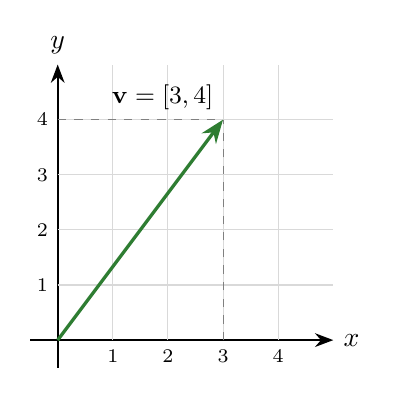
\begin{tikzpicture}[scale=0.7]
    % Axes
    \draw[-{Stealth}, thick] (-0.5, 0) -- (5, 0) node[right] {$x$};
    \draw[-{Stealth}, thick] (0, -0.5) -- (0, 5) node[above] {$y$};
    % Grid
    \foreach \x in {1,2,3,4} {
        \draw[gray!30] (\x, 0) -- (\x, 5);
        \draw[gray!30] (0, \x) -- (5, \x);
        \node[below, font=\scriptsize] at (\x, 0) {\x};
        \node[left, font=\scriptsize] at (0, \x) {\x};
    }
    % Vector
    \draw[-{Stealth[length=3mm]}, very thick, alfaisalgreen] (0,0) -- (3,4);
    \node[above left, font=\small\bfseries] at (3,4) {$\mathbf{v} = [3, 4]$};
    % Dashed projections
    \draw[dashed, gray] (3, 0) -- (3, 4);
    \draw[dashed, gray] (0, 4) -- (3, 4);
\end{tikzpicture}
\end{center}

\subsection{3D Vectors}

A \textbf{3D vector} extends to three dimensions: $\mathbf{v} = [x, y, z]$. In practice, vectors in AI are often hundreds or thousands of dimensions, but the same principles apply.

\subsection{Representing Vectors in NumPy}

Python's \texttt{NumPy} library is the standard tool for working with vectors:

\begin{lstlisting}[language=Python]
import numpy as np

# 2D vector
v_2d = np.array([3, 4])

# 3D vector
v_3d = np.array([1, 2, 3])

# High-dimensional vector (common in NLP)
v_embed = np.array([0.2, -0.4, 0.7, 0.3, -0.1, 0.8, 0.5, -0.2])
\end{lstlisting}

\subsection{Feature Vectors}

In AI, a \textbf{feature vector} is an ordered list of numbers where each position represents a specific attribute of the data. For example, to represent a house for a price-prediction model:

\[
\mathbf{x}_{\text{house}} = [\underbrace{150}_{\text{area (m}^2\text{)}},\; \underbrace{3}_{\text{bedrooms}},\; \underbrace{2}_{\text{bathrooms}},\; \underbrace{5}_{\text{age (years)}},\; \underbrace{1}_{\text{garage (yes)}}]
\]

\begin{tcolorbox}[warnbox={Important}]
The \textbf{order} matters in a feature vector. Swapping two values changes the meaning entirely. All vectors in a dataset must follow the \textbf{same convention} for which position encodes which feature.
\end{tcolorbox}

% ============================================================
% 2. VECTOR OPERATIONS
% ============================================================
\section{Vector Operations}

\subsection{Addition and Subtraction}

Vector addition and subtraction are performed \textbf{element-wise}:

\medskip\noindent\textbf{Worked Example:}

Let $\mathbf{v} = [2, 4, 6]$ and $\mathbf{w} = [1, 0, 1]$.

\[
\mathbf{v} + \mathbf{w} = [2+1,\; 4+0,\; 6+1] = [3, 4, 7]
\]
\[
\mathbf{v} - \mathbf{w} = [2-1,\; 4-0,\; 6-1] = [1, 4, 5]
\]

\begin{center}
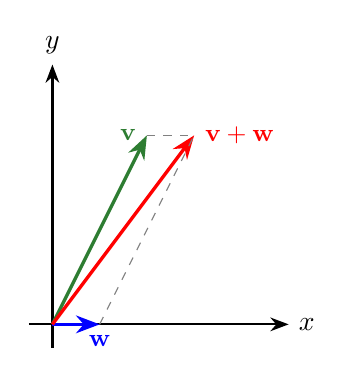
\begin{tikzpicture}[scale=0.6]
    % Axes
    \draw[-{Stealth}, thick] (-0.5, 0) -- (5, 0) node[right] {$x$};
    \draw[-{Stealth}, thick] (0, -0.5) -- (0, 5.5) node[above] {$y$};
    % Vectors (projecting to 2D: use first two components)
    \draw[-{Stealth[length=3mm]}, very thick, alfaisalgreen] (0,0) -- (2,4) node[left, font=\small] {$\mathbf{v}$};
    \draw[-{Stealth[length=3mm]}, very thick, blue] (0,0) -- (1,0) node[below, font=\small] {$\mathbf{w}$};
    \draw[-{Stealth[length=3mm]}, very thick, red] (0,0) -- (3,4) node[right, font=\small] {$\mathbf{v}+\mathbf{w}$};
    % Parallelogram
    \draw[dashed, gray] (2,4) -- (3,4);
    \draw[dashed, gray] (1,0) -- (3,4);
\end{tikzpicture}
\end{center}

\textit{Geometric intuition:} Vector addition follows the \textbf{parallelogram rule}---place the tail of $\mathbf{w}$ at the head of $\mathbf{v}$, and the result is the diagonal.

\subsection{Scalar Multiplication}

Multiplying a vector by a scalar (a single number) scales every element:

\medskip\noindent\textbf{Worked Example:}

Let $c = 3$ and $\mathbf{v} = [2, 4, 6]$.

\[
c \cdot \mathbf{v} = 3 \cdot [2, 4, 6] = [6, 12, 18]
\]

\textit{Geometric intuition:} Scalar multiplication \textbf{stretches} (if $|c| > 1$) or \textbf{shrinks} (if $|c| < 1$) the vector. A negative scalar \textbf{reverses} the direction.

\begin{lstlisting}[language=Python]
import numpy as np

v = np.array([2, 4, 6])
w = np.array([1, 0, 1])

print(v + w)      # [3, 4, 7]
print(v - w)      # [1, 4, 5]
print(3 * v)      # [ 6, 12, 18]
\end{lstlisting}

\begin{tcolorbox}[questionbox={Self-Check Q1}]
Given $\mathbf{a} = [1, -2, 3]$ and $\mathbf{b} = [4, 0, -1]$, compute $2\mathbf{a} + \mathbf{b}$ and $\mathbf{a} - 3\mathbf{b}$. \textit{(Solution in Appendix)}
\end{tcolorbox}

% ============================================================
% 3. VECTORS IN COMPUTER VISION
% ============================================================
\section{Vectors in Computer Vision}

\subsection{Images as Matrices of Pixel Values}

A digital image is fundamentally a \textbf{matrix of numbers}. Each number represents the brightness (or color intensity) of a single pixel:

\begin{itemize}[leftmargin=1.5em]
    \item \textbf{Pixel values} range from \texttt{0} (black) to \texttt{255} (white)
    \item \textbf{Grayscale image}: a single 2D array of shape $H \times W$
    \item \textbf{Color (RGB) image}: three 2D arrays stacked together, shape $H \times W \times 3$ (one channel each for Red, Green, Blue)
\end{itemize}

\subsection{Example: A 2$\times$2 Grayscale Image}

Consider a tiny 2$\times$2 image with a checkerboard pattern:

\[
\text{Image} = \begin{bmatrix} 0 & 255 \\ 255 & 0 \end{bmatrix}
\]

\begin{itemize}[leftmargin=1.5em]
    \item Top-left pixel: 0 (black)
    \item Top-right pixel: 255 (white)
    \item Bottom-left pixel: 255 (white)
    \item Bottom-right pixel: 0 (black)
\end{itemize}

\begin{lstlisting}[language=Python]
import numpy as np

# A 2x2 grayscale image (checkerboard)
image = np.array([[0, 255],
                  [255, 0]])

print(image.shape)   # (2, 2)
print(image.dtype)   # int64
\end{lstlisting}

\subsection{Color Images as 3D Tensors}

A color image has three channels. For a 4$\times$4 RGB image:

\begin{lstlisting}[language=Python]
# Shape: (height, width, channels)
rgb_image = np.random.randint(0, 256, size=(4, 4, 3))
print(rgb_image.shape)  # (4, 4, 3)
\end{lstlisting}

\begin{tcolorbox}[intuitionbox={Key Insight}]
An image of size $224 \times 224 \times 3$ (a common input size for CNNs) is ultimately a vector of $224 \times 224 \times 3 = 150{,}528$ numbers. AI models process images by treating these numbers as input features---the same principle as feature vectors, just with many more dimensions.
\end{tcolorbox}

% ============================================================
% 4. VECTORS IN NLP
% ============================================================
\section{Vectors in NLP: Words as Vectors}

\subsection{Word Embeddings}

In NLP, each word is mapped to a dense vector called a \textbf{word embedding}. Unlike raw text, these vectors capture \textbf{semantic meaning}:

\begin{lstlisting}[language=Python]
import numpy as np

# A 4-dimensional word embedding for "king"
king = np.array([0.2, -0.4, 0.7, 0.3])
\end{lstlisting}

Each dimension encodes some abstract linguistic feature (e.g., gender, royalty, animacy). These features are \textbf{learned automatically} from data---they are not hand-designed.

\subsection{Similar Words Have Similar Vectors}

The fundamental property of word embeddings is that \textbf{semantically similar words are close together} in the vector space:

\begin{center}
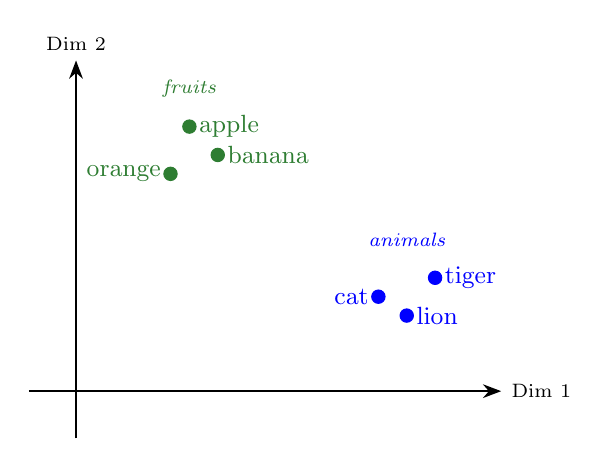
\begin{tikzpicture}[scale=1.2]
    % Axes
    \draw[-{Stealth}, thick] (-0.5, 0) -- (4.5, 0) node[right] {\scriptsize Dim 1};
    \draw[-{Stealth}, thick] (0, -0.5) -- (0, 3.5) node[above] {\scriptsize Dim 2};
    % Words - fruits cluster
    \filldraw[alfaisalgreen] (1.2, 2.8) circle (2pt) node[right, font=\small] {apple};
    \filldraw[alfaisalgreen] (1.5, 2.5) circle (2pt) node[right, font=\small] {banana};
    \filldraw[alfaisalgreen] (1.0, 2.3) circle (2pt) node[left, font=\small] {orange};
    % Words - animals cluster
    \filldraw[blue] (3.5, 0.8) circle (2pt) node[right, font=\small] {lion};
    \filldraw[blue] (3.8, 1.2) circle (2pt) node[right, font=\small] {tiger};
    \filldraw[blue] (3.2, 1.0) circle (2pt) node[left, font=\small] {cat};
    % Labels
    \node[font=\scriptsize\itshape, alfaisalgreen] at (1.2, 3.2) {fruits};
    \node[font=\scriptsize\itshape, blue] at (3.5, 1.6) {animals};
\end{tikzpicture}
\end{center}

\subsection{Using spaCy to Get Embeddings}

\begin{lstlisting}[language=Python]
import spacy
nlp = spacy.load("en_core_web_md")

apple  = nlp("apple").vector
banana = nlp("banana").vector
lion   = nlp("lion").vector

print(apple.shape)  # (300,)  -- 300-dimensional vector
\end{lstlisting}

\subsection{Measuring Word Similarity with Dot Product}

We can use the \textbf{dot product} to quantify similarity between word vectors:

\begin{lstlisting}[language=Python]
# Dot product: higher = more similar
sim_fruit = np.dot(apple, banana)   # high value (similar)
sim_diff  = np.dot(apple, lion)     # lower value (dissimilar)

print(f"apple . banana = {sim_fruit:.2f}")
print(f"apple . lion   = {sim_diff:.2f}")
\end{lstlisting}

\begin{tcolorbox}[intuitionbox={Intuition}]
Words that appear in similar contexts (``I ate an \textit{apple}'' vs.\ ``I ate a \textit{banana}'') end up with similar vectors. Words from different semantic domains (``apple'' vs.\ ``lion'') end up far apart. This is the distributional hypothesis: \textit{``You shall know a word by the company it keeps''} (Firth, 1957).
\end{tcolorbox}

\begin{tcolorbox}[questionbox={Self-Check Q2}]
Why do word embeddings typically have 100--300 dimensions instead of, say, 3 or 10{,}000? What are the trade-offs? \textit{(Solution in Appendix)}
\end{tcolorbox}

% ============================================================
% 5. DOT PRODUCT
% ============================================================
\section{The Dot Product}

\subsection{Definition}

The \textbf{dot product} (also called the \textbf{inner product}) of two vectors $\mathbf{x}$ and $\mathbf{y}$ of length $n$ is:

\begin{equation}
\boxed{\mathbf{x} \cdot \mathbf{y} = \sum_{i=1}^{n} x_i \cdot y_i = x_1 y_1 + x_2 y_2 + \cdots + x_n y_n}
\end{equation}

The dot product takes two vectors and returns a \textbf{single number} (a scalar).

\subsection{Worked Example}

Let $\mathbf{x} = [2, 3, 4]$ and $\mathbf{y} = [1, 0, -1]$.

\[
\mathbf{x} \cdot \mathbf{y} = (2)(1) + (3)(0) + (4)(-1) = 2 + 0 - 4 = -2
\]

\begin{lstlisting}[language=Python]
import numpy as np

x = np.array([2, 3, 4])
y = np.array([1, 0, -1])

print(np.dot(x, y))  # -2
\end{lstlisting}

\subsection{Properties}

\begin{itemize}[leftmargin=1.5em]
    \item \textbf{Commutative:} $\mathbf{x} \cdot \mathbf{y} = \mathbf{y} \cdot \mathbf{x}$
    \item \textbf{Distributive:} $\mathbf{x} \cdot (\mathbf{y} + \mathbf{z}) = \mathbf{x} \cdot \mathbf{y} + \mathbf{x} \cdot \mathbf{z}$
    \item \textbf{Scalar factor:} $(c\,\mathbf{x}) \cdot \mathbf{y} = c\,(\mathbf{x} \cdot \mathbf{y})$
\end{itemize}

\subsection{Geometric Meaning: Measuring Alignment}

The dot product has a powerful geometric interpretation:

\begin{equation}
\mathbf{x} \cdot \mathbf{y} = \|\mathbf{x}\| \cdot \|\mathbf{y}\| \cdot \cos\theta
\end{equation}

where $\theta$ is the angle between the two vectors. This tells us:

\begin{center}
\renewcommand{\arraystretch}{1.4}
\begin{tabular}{@{}lccl@{}}
\toprule
\textbf{Case} & \textbf{Angle} & \textbf{Dot Product} & \textbf{Meaning} \\
\midrule
Same direction & $\theta = 0^\circ$ & Maximum (positive) & Perfectly aligned \\
Perpendicular & $\theta = 90^\circ$ & 0 & No relationship \\
Opposite direction & $\theta = 180^\circ$ & Maximum (negative) & Perfectly opposed \\
Some angle & $0^\circ < \theta < 90^\circ$ & Positive & Partially aligned \\
\bottomrule
\end{tabular}
\end{center}

\begin{center}
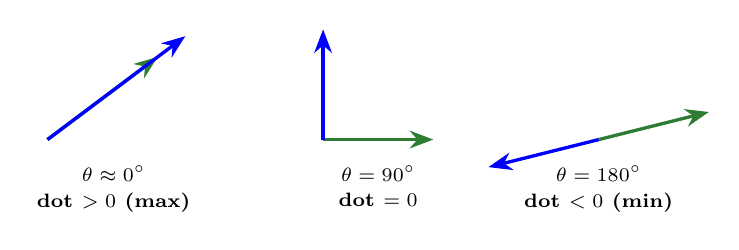
\begin{tikzpicture}[scale=0.7]
    % Case 1: same direction
    \begin{scope}[shift={(0,0)}]
        \draw[-{Stealth[length=3mm]}, very thick, alfaisalgreen] (0,0) -- (2,1.5);
        \draw[-{Stealth[length=3mm]}, very thick, blue] (0,0) -- (2.5,1.875);
        \node[font=\scriptsize, below] at (1.2, -0.3) {$\theta \approx 0^\circ$};
        \node[font=\scriptsize\bfseries, below] at (1.2, -0.8) {dot $> 0$ (max)};
    \end{scope}
    % Case 2: perpendicular
    \begin{scope}[shift={(5,0)}]
        \draw[-{Stealth[length=3mm]}, very thick, alfaisalgreen] (0,0) -- (2,0);
        \draw[-{Stealth[length=3mm]}, very thick, blue] (0,0) -- (0,2);
        \node[font=\scriptsize, below] at (1, -0.3) {$\theta = 90^\circ$};
        \node[font=\scriptsize\bfseries, below] at (1, -0.8) {dot $= 0$};
    \end{scope}
    % Case 3: opposite
    \begin{scope}[shift={(10,0)}]
        \draw[-{Stealth[length=3mm]}, very thick, alfaisalgreen] (0,0) -- (2,0.5);
        \draw[-{Stealth[length=3mm]}, very thick, blue] (0,0) -- (-2,-0.5);
        \node[font=\scriptsize, below] at (0, -0.3) {$\theta = 180^\circ$};
        \node[font=\scriptsize\bfseries, below] at (0, -0.8) {dot $< 0$ (min)};
    \end{scope}
\end{tikzpicture}
\end{center}

\begin{tcolorbox}[intuitionbox={Why This Matters for NLP}]
In word embeddings, the dot product measures how ``aligned'' two word meanings are. A high positive dot product means the words are semantically similar. A dot product near zero means they are unrelated. A negative dot product means they are semantically opposed.
\end{tcolorbox}

\begin{tcolorbox}[questionbox={Self-Check Q3}]
Compute the dot product of $\mathbf{a} = [1, 2, 3]$ and $\mathbf{b} = [4, -5, 6]$. Are these vectors more aligned, perpendicular, or opposed? \textit{(Solution in Appendix)}
\end{tcolorbox}

% ============================================================
% 6. VECTOR NORMALIZATION
% ============================================================
\section{Vector Normalization}

\subsection{Why Normalize?}

Consider two word vectors:
\begin{itemize}[leftmargin=1.5em]
    \item $\mathbf{a} = [100, 200]$ (a word that appears 1000 times in the corpus)
    \item $\mathbf{b} = [1, 2]$ (a rare word)
\end{itemize}

Their dot product $\mathbf{a} \cdot \mathbf{b} = 500$ is large simply because $\mathbf{a}$ has large values, not because they are particularly similar. \textbf{Normalization} removes the effect of magnitude so we can compare \textbf{directions only}.

\subsection{L2 Norm (Euclidean Norm)}

The \textbf{L2 norm} measures the ``length'' of a vector:

\begin{equation}
\boxed{\|\mathbf{x}\|_2 = \sqrt{\sum_{i=1}^{n} x_i^2} = \sqrt{x_1^2 + x_2^2 + \cdots + x_n^2}}
\end{equation}

\medskip\noindent\textbf{Worked Example:}

Let $\mathbf{v} = [3, 4]$.

\[
\|\mathbf{v}\|_2 = \sqrt{3^2 + 4^2} = \sqrt{9 + 16} = \sqrt{25} = 5
\]

\textbf{Normalized vector} (unit vector):

\[
\hat{\mathbf{v}} = \frac{\mathbf{v}}{\|\mathbf{v}\|_2} = \frac{[3, 4]}{5} = [0.6,\; 0.8]
\]

The normalized vector has length 1: $\sqrt{0.6^2 + 0.8^2} = \sqrt{0.36 + 0.64} = 1$.

\begin{lstlisting}[language=Python]
import numpy as np

v = np.array([3, 4])
norm = np.linalg.norm(v)          # 5.0
v_normalized = v / norm            # [0.6, 0.8]
print(np.linalg.norm(v_normalized))  # 1.0
\end{lstlisting}

\subsection{L1 Norm (Manhattan Norm)}

The \textbf{L1 norm} sums the absolute values:

\begin{equation}
\boxed{\|\mathbf{x}\|_1 = \sum_{i=1}^{n} |x_i| = |x_1| + |x_2| + \cdots + |x_n|}
\end{equation}

\medskip\noindent\textbf{Example:} $\mathbf{v} = [3, -4]$, then $\|\mathbf{v}\|_1 = |3| + |-4| = 7$.

\subsection{When to Use Which Norm}

\begin{center}
\renewcommand{\arraystretch}{1.3}
\begin{tabular}{@{}lll@{}}
\toprule
\textbf{Norm} & \textbf{Geometric Meaning} & \textbf{Common Use} \\
\midrule
L2 (Euclidean) & Straight-line distance & Cosine similarity, embeddings \\
L1 (Manhattan) & City-block distance & Sparse models, regularization \\
\bottomrule
\end{tabular}
\end{center}

\begin{tcolorbox}[warnbox={Key Point}]
After L2 normalization, every vector has length 1. This means the dot product of two normalized vectors equals their \textbf{cosine similarity}---it measures only the \textbf{angle} between vectors, ignoring magnitude.
\end{tcolorbox}

\begin{tcolorbox}[questionbox={Self-Check Q4}]
Compute the L2 norm and the L1 norm of $\mathbf{u} = [1, -2, 2]$. Then normalize $\mathbf{u}$ using the L2 norm. \textit{(Solution in Appendix)}
\end{tcolorbox}

% ============================================================
% 7. COSINE SIMILARITY
% ============================================================
\section{Cosine Similarity}

\subsection{Definition}

\textbf{Cosine similarity} measures the cosine of the angle between two vectors, giving a value between $-1$ and $+1$:

\begin{equation}
\boxed{\text{cos\_sim}(\mathbf{x}, \mathbf{y}) = \frac{\mathbf{x} \cdot \mathbf{y}}{\|\mathbf{x}\|_2 \cdot \|\mathbf{y}\|_2} = \frac{\displaystyle\sum_{i=1}^{n} x_i y_i}{\sqrt{\displaystyle\sum_{i=1}^{n} x_i^2} \;\cdot\; \sqrt{\displaystyle\sum_{i=1}^{n} y_i^2}}}
\end{equation}

\begin{center}
\renewcommand{\arraystretch}{1.3}
\begin{tabular}{@{}cll@{}}
\toprule
\textbf{Value} & \textbf{Meaning} & \textbf{Example} \\
\midrule
$+1$ & Identical direction & ``happy'' and ``joyful'' \\
$0$ & Orthogonal (unrelated) & ``happy'' and ``table'' \\
$-1$ & Opposite direction & ``happy'' and ``sad'' \\
\bottomrule
\end{tabular}
\end{center}

\subsection{Worked Example}

Let $\mathbf{a} = [3, 4]$ and $\mathbf{b} = [4, 3]$.

\medskip\noindent\textbf{Step 1:} Dot product.
\[
\mathbf{a} \cdot \mathbf{b} = (3)(4) + (4)(3) = 12 + 12 = 24
\]

\noindent\textbf{Step 2:} Norms.
\[
\|\mathbf{a}\|_2 = \sqrt{9 + 16} = 5, \qquad \|\mathbf{b}\|_2 = \sqrt{16 + 9} = 5
\]

\noindent\textbf{Step 3:} Cosine similarity.
\[
\text{cos\_sim}(\mathbf{a}, \mathbf{b}) = \frac{24}{5 \times 5} = \frac{24}{25} = 0.96
\]

This is very close to 1, meaning $\mathbf{a}$ and $\mathbf{b}$ point in nearly the same direction.

\begin{lstlisting}[language=Python]
import numpy as np

a = np.array([3, 4])
b = np.array([4, 3])

cos_sim = np.dot(a, b) / (np.linalg.norm(a) * np.linalg.norm(b))
print(f"Cosine similarity: {cos_sim:.4f}")  # 0.9600
\end{lstlisting}

\subsection{Why Cosine Similarity Matters}

\begin{tcolorbox}[intuitionbox={Direction vs.\ Magnitude}]
Cosine similarity measures how similar two vectors are \textbf{in direction}, regardless of their magnitude. This is crucial because:
\begin{itemize}[leftmargin=1em, itemsep=2pt]
    \item A document about ``cats'' that is 10 pages long should be as similar to another ``cats'' document as one that is 2 pages long---they point in the same direction even though the longer document has larger vector magnitude.
    \item Word frequency differences should not affect semantic similarity comparisons.
\end{itemize}
\end{tcolorbox}

\subsection{Applications}

\begin{itemize}[leftmargin=1.5em]
    \item \textbf{Document similarity:} Represent documents as vectors (e.g., TF-IDF), compare with cosine similarity
    \item \textbf{Word similarity:} Compare word embeddings to find synonyms
    \item \textbf{Search engines:} Rank documents by cosine similarity to the query vector
    \item \textbf{Recommendation systems:} Find users/items with similar preference vectors
\end{itemize}

\begin{tcolorbox}[questionbox={Self-Check Q5}]
Compute the cosine similarity between $\mathbf{p} = [1, 0, -1]$ and $\mathbf{q} = [-1, 0, 1]$. What does the result tell you about the relationship between these vectors? \textit{(Solution in Appendix)}
\end{tcolorbox}

% ============================================================
% 8. FROM VECTORS TO WORD EMBEDDINGS
% ============================================================
\section{From Vectors to Word Embeddings}

\subsection{The Big Picture}

Now that we understand vectors and similarity measures, we can address the central question: \textbf{How do we convert words into meaningful vectors?}

There are two major approaches:

\subsubsection*{Approach 1: One-Hot Encoding (Naive)}

Each word is represented as a vector with a single 1 and all other entries 0:

\[
\text{``cat''} = [1, 0, 0, 0, \ldots, 0], \quad \text{``dog''} = [0, 1, 0, 0, \ldots, 0], \quad \text{``fish''} = [0, 0, 1, 0, \ldots, 0]
\]

\begin{tcolorbox}[warnbox={Problems with One-Hot Encoding}]
\begin{itemize}[leftmargin=1em, itemsep=2pt]
    \item \textbf{Huge dimensionality:} Vocabulary of 50{,}000 words $\to$ each vector has 50{,}000 dimensions
    \item \textbf{Sparse:} Almost all entries are 0 (wasteful)
    \item \textbf{No semantics:} $\text{cos\_sim}(\text{``cat''}, \text{``dog''}) = 0$ --- same as $\text{cos\_sim}(\text{``cat''}, \text{``refrigerator''}) = 0$. The model cannot tell that cats and dogs are more related than cats and refrigerators.
\end{itemize}
\end{tcolorbox}

\subsubsection*{Approach 2: Dense Embeddings (Modern)}

Each word is mapped to a \textbf{low-dimensional, dense vector} (typically 100--300 dimensions) that captures semantic meaning. These vectors are \textbf{learned from data}.

\[
\text{``cat''} = [0.2, -0.4, 0.7, \ldots], \quad \text{``dog''} = [0.25, -0.38, 0.65, \ldots]
\]

Now $\text{cos\_sim}(\text{``cat''}, \text{``dog''}) \approx 0.85$ --- the model understands they are related.

\subsection{Word2Vec}

\textbf{Word2Vec} (Mikolov et al., 2013) learns word embeddings by training a shallow neural network on a simple prediction task. It has two variants:

\subsubsection*{CBOW (Continuous Bag of Words)}

Predict the \textbf{center word} from surrounding context words:

\begin{center}
Context: ``The \underline{\hspace{1cm}} sat on the mat'' $\to$ Predict: ``cat''
\end{center}

\subsubsection*{Skip-gram}

Predict the \textbf{context words} from the center word:

\begin{center}
Input: ``cat'' $\to$ Predict: ``The'', ``sat'', ``on'', ``the'', ``mat''
\end{center}

\begin{tcolorbox}[intuitionbox={The Famous Analogy}]
Word2Vec captures remarkable semantic relationships through vector arithmetic:
\[
\vec{\text{king}} - \vec{\text{man}} + \vec{\text{woman}} \approx \vec{\text{queen}}
\]
This works because the model learns that the ``royalty'' and ``gender'' dimensions are independent, so subtracting ``man'' removes the male component, and adding ``woman'' adds the female component.
\end{tcolorbox}

\subsection{GloVe (Global Vectors)}

\textbf{GloVe} (Pennington et al., 2014) takes a different approach: instead of predicting context words, it factorizes the \textbf{global word co-occurrence matrix}. If ``ice'' and ``cold'' frequently appear together across the entire corpus, GloVe ensures their vectors are close.

\begin{itemize}[leftmargin=1.5em]
    \item \textbf{Advantage:} Captures global corpus statistics, not just local windows
    \item \textbf{Result:} Often produces high-quality embeddings for common words
\end{itemize}

\subsection{fastText}

\textbf{fastText} (Bojanowski et al., 2017) extends Word2Vec by representing each word as a \textbf{bag of character n-grams} (subwords). For example, ``where'' with $n=3$:

\[
\text{``where''} \to \{\text{``<wh''}, \text{``whe''}, \text{``her''}, \text{``ere''}, \text{``re>''}\}
\]

\begin{itemize}[leftmargin=1.5em]
    \item \textbf{Advantage:} Can generate vectors for \textbf{out-of-vocabulary} (OOV) words by composing subword vectors
    \item \textbf{Example:} Even if ``unfriendliness'' was never seen during training, fastText can construct its vector from subwords like ``un'', ``friend'', ``li'', ``ness''
\end{itemize}

\subsection{Comparison of Embedding Methods}

\begin{center}
\renewcommand{\arraystretch}{1.4}
\begin{tabular}{@{}p{2.5cm}p{3cm}p{3cm}p{3cm}@{}}
\toprule
& \textbf{Word2Vec} & \textbf{GloVe} & \textbf{fastText} \\
\midrule
\textbf{Training} & Predict context (local windows) & Co-occurrence matrix (global) & Predict context + subwords \\
\textbf{OOV words} & Cannot handle & Cannot handle & Handles via subwords \\
\textbf{Morphology} & Ignores & Ignores & Captures (``run'', ``running'') \\
\textbf{Speed} & Fast & Medium & Fast \\
\textbf{Best for} & General use & Large corpora & Morphologically rich languages \\
\bottomrule
\end{tabular}
\end{center}

\begin{tcolorbox}[warnbox={Limitation of All Three Methods}]
Word2Vec, GloVe, and fastText all produce \textbf{static embeddings}: each word gets one fixed vector regardless of context. The word ``bank'' has the same vector whether it means a financial institution or a riverbank. Solving this limitation requires \textbf{contextual embeddings} (ELMo, BERT, GPT), which are the subject of Lecture~4.
\end{tcolorbox}

\begin{tcolorbox}[questionbox={Self-Check Q6}]
Explain why the analogy $\vec{\text{king}} - \vec{\text{man}} + \vec{\text{woman}} \approx \vec{\text{queen}}$ works in Word2Vec. What geometric property of the embedding space does this exploit? \textit{(Solution in Appendix)}
\end{tcolorbox}

% ============================================================
% 9. SUMMARY
% ============================================================
\section{Summary: The Vector Foundation for NLP}

This lecture established the \textbf{mathematical foundation} that underpins all of modern NLP:

\begin{center}
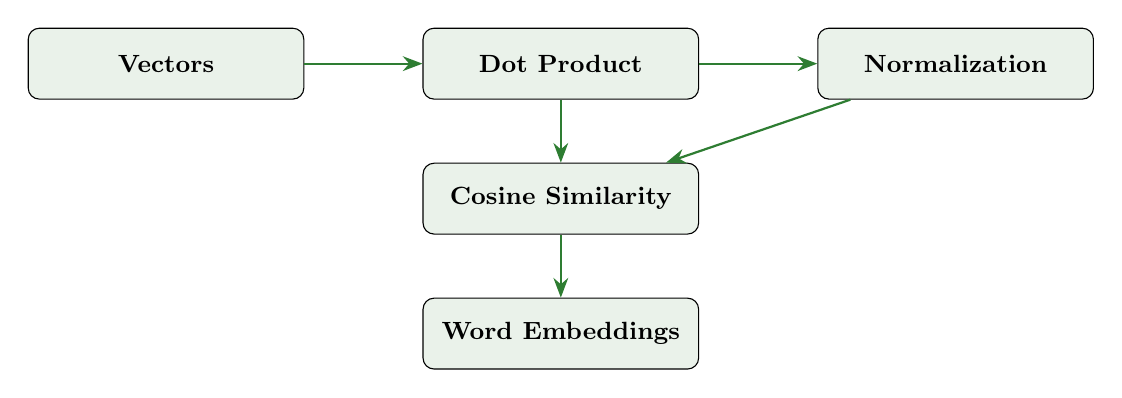
\begin{tikzpicture}[
    node distance=0.8cm,
    box/.style={draw, rounded corners, minimum height=0.9cm, minimum width=3.5cm, font=\small\bfseries, align=center, fill=alfaisalgreen!10},
    arr/.style={-{Stealth[length=2.5mm]}, thick, alfaisalgreen}
]
\node[box] (vec) {Vectors};
\node[box, right=1.5cm of vec] (ops) {Dot Product};
\node[box, right=1.5cm of ops] (norm) {Normalization};
\node[box, below=of ops] (cos) {Cosine Similarity};
\node[box, below=of cos] (emb) {Word Embeddings};

\draw[arr] (vec) -- (ops);
\draw[arr] (ops) -- (norm);
\draw[arr] (ops) -- (cos);
\draw[arr] (norm) -- (cos);
\draw[arr] (cos) -- (emb);
\end{tikzpicture}
\end{center}

\subsection{Key Takeaways}

\begin{enumerate}[leftmargin=1.5em]
    \item \textbf{Vectors} are the universal representation for all data in AI---text, images, audio.
    \item \textbf{Vector operations} (addition, subtraction, scalar multiplication) enable arithmetic on meanings.
    \item The \textbf{dot product} measures alignment between vectors; it is the core operation of similarity computation.
    \item \textbf{Normalization} removes magnitude effects, enabling fair direction-based comparison.
    \item \textbf{Cosine similarity} combines dot product and normalization to give a principled similarity measure in $[-1, 1]$.
    \item \textbf{Word embeddings} (Word2Vec, GloVe, fastText) use these mathematical tools to map words into meaningful vector spaces where similar words are close together.
    \item All these methods produce \textbf{static} embeddings. \textbf{Contextual} embeddings (Lecture~4) will address the limitation that each word gets a single fixed vector.
\end{enumerate}

\begin{tcolorbox}[questionbox={Self-Check Q7}]
A search engine represents both documents and queries as vectors. Explain step by step how it uses the concepts from this lecture to rank documents by relevance to a query. \textit{(Solution in Appendix)}
\end{tcolorbox}

% ============================================================
% APPENDIX
% ============================================================
\newpage
\section*{Appendix: Solutions to Self-Check Questions}
\addcontentsline{toc}{section}{Appendix: Solutions to Self-Check Questions}

\subsection*{Q1: Compute $2\mathbf{a} + \mathbf{b}$ and $\mathbf{a} - 3\mathbf{b}$}

Given $\mathbf{a} = [1, -2, 3]$ and $\mathbf{b} = [4, 0, -1]$:

\medskip
$2\mathbf{a} + \mathbf{b}$:
\[
2\mathbf{a} = [2, -4, 6], \qquad 2\mathbf{a} + \mathbf{b} = [2+4,\; -4+0,\; 6+(-1)] = [6, -4, 5]
\]

$\mathbf{a} - 3\mathbf{b}$:
\[
3\mathbf{b} = [12, 0, -3], \qquad \mathbf{a} - 3\mathbf{b} = [1-12,\; -2-0,\; 3-(-3)] = [-11, -2, 6]
\]

\subsection*{Q2: Why 100--300 dimensions for word embeddings?}

This is a balance between \textbf{expressiveness} and \textbf{efficiency}:

\begin{itemize}[leftmargin=1.5em]
    \item \textbf{Too few dimensions (e.g., 3--10):} Not enough capacity to capture the rich semantic relationships among tens of thousands of words. Different meanings would ``collide'' in the same region of space.
    \item \textbf{Too many dimensions (e.g., 10{,}000):} The model has more parameters to learn, requiring much more training data and computation. It also risks overfitting---memorizing the training data rather than learning general patterns. Additionally, high-dimensional spaces suffer from the \textbf{curse of dimensionality}: distances between points become less meaningful.
    \item \textbf{100--300 dimensions:} Empirically found to be the sweet spot---enough capacity to represent nuanced semantic relationships while remaining computationally tractable.
\end{itemize}

\subsection*{Q3: Dot product of $\mathbf{a} = [1, 2, 3]$ and $\mathbf{b} = [4, -5, 6]$}

\[
\mathbf{a} \cdot \mathbf{b} = (1)(4) + (2)(-5) + (3)(6) = 4 - 10 + 18 = 12
\]

Since the dot product is \textbf{positive}, the vectors are \textbf{partially aligned} (the angle between them is less than $90^\circ$). They are not perfectly aligned (which would require them to point in exactly the same direction) but they are more similar than different.

\subsection*{Q4: L2 norm, L1 norm, and normalization of $\mathbf{u} = [1, -2, 2]$}

\textbf{L2 norm:}
\[
\|\mathbf{u}\|_2 = \sqrt{1^2 + (-2)^2 + 2^2} = \sqrt{1 + 4 + 4} = \sqrt{9} = 3
\]

\textbf{L1 norm:}
\[
\|\mathbf{u}\|_1 = |1| + |-2| + |2| = 1 + 2 + 2 = 5
\]

\textbf{L2-normalized vector:}
\[
\hat{\mathbf{u}} = \frac{\mathbf{u}}{\|\mathbf{u}\|_2} = \frac{[1, -2, 2]}{3} = \left[\frac{1}{3},\; -\frac{2}{3},\; \frac{2}{3}\right] \approx [0.333, -0.667, 0.667]
\]

Verification: $\sqrt{(1/3)^2 + (-2/3)^2 + (2/3)^2} = \sqrt{1/9 + 4/9 + 4/9} = \sqrt{9/9} = 1$. \checkmark

\subsection*{Q5: Cosine similarity of $\mathbf{p} = [1, 0, -1]$ and $\mathbf{q} = [-1, 0, 1]$}

\textbf{Dot product:}
\[
\mathbf{p} \cdot \mathbf{q} = (1)(-1) + (0)(0) + (-1)(1) = -1 + 0 - 1 = -2
\]

\textbf{Norms:}
\[
\|\mathbf{p}\|_2 = \sqrt{1 + 0 + 1} = \sqrt{2}, \qquad \|\mathbf{q}\|_2 = \sqrt{1 + 0 + 1} = \sqrt{2}
\]

\textbf{Cosine similarity:}
\[
\text{cos\_sim}(\mathbf{p}, \mathbf{q}) = \frac{-2}{\sqrt{2} \cdot \sqrt{2}} = \frac{-2}{2} = -1
\]

A cosine similarity of $-1$ means the vectors point in \textbf{exactly opposite directions}. $\mathbf{q} = -\mathbf{p}$, so they are perfectly anti-correlated. In an NLP context, this would mean the two items have maximally opposite meanings (though in practice, cosine similarities of exactly $-1$ are rare for word embeddings).

\subsection*{Q6: Why does king $-$ man $+$ woman $\approx$ queen?}

Word2Vec learns an embedding space where \textbf{semantic relationships correspond to consistent vector offsets}. The key geometric property is that analogous relationships form \textbf{parallelograms} in the vector space:

\begin{itemize}[leftmargin=1.5em]
    \item The vector from ``man'' to ``king'' captures the concept of \textbf{royalty}: $\vec{\text{king}} - \vec{\text{man}} \approx \vec{\text{royalty}}$
    \item The vector from ``woman'' to ``queen'' captures the \textbf{same concept}: $\vec{\text{queen}} - \vec{\text{woman}} \approx \vec{\text{royalty}}$
    \item Therefore: $\vec{\text{king}} - \vec{\text{man}} \approx \vec{\text{queen}} - \vec{\text{woman}}$
    \item Rearranging: $\vec{\text{king}} - \vec{\text{man}} + \vec{\text{woman}} \approx \vec{\text{queen}}$
\end{itemize}

This works because the embedding space organizes words such that semantic dimensions (gender, royalty, tense, etc.) are \textbf{approximately linear and additive}. This is an emergent property of training on large corpora---the model discovers these axes of meaning automatically.

\subsection*{Q7: How a search engine uses these concepts}

A vector-based search engine works as follows:

\begin{enumerate}[leftmargin=1.5em]
    \item \textbf{Vectorize documents:} Each document in the collection is converted into a vector. This can be done using TF-IDF (term frequency--inverse document frequency) or by averaging word embeddings for all words in the document.
    \item \textbf{Vectorize the query:} The user's search query is converted into a vector using the same method.
    \item \textbf{Normalize:} Both document vectors and the query vector are L2-normalized so that document length does not bias the results (a 100-page document about cats should not outrank a 2-page document about cats just because it is longer).
    \item \textbf{Compute cosine similarity:} For each document, compute $\text{cos\_sim}(\vec{q}, \vec{d})$. Since both vectors are normalized, this is simply the dot product $\vec{q} \cdot \vec{d}$.
    \item \textbf{Rank:} Sort documents by cosine similarity in descending order. The document with the highest cosine similarity is the most relevant to the query.
    \item \textbf{Return top-$k$:} Present the top-$k$ ranked documents to the user.
\end{enumerate}

This approach captures \textbf{semantic relevance} (not just keyword matching) because the embedding vectors encode meaning, and cosine similarity measures how closely that meaning aligns between query and document.

\end{document}
